% !TEX root = main.tex
\chapter{Acoustic model training}
\label{cha:train}

This chapter present new Kaldi acoustic modeling recipe for free Czech and English data.
The recipe scripts were developed as part of this thesis and are licensed under the Apache 2.0 license and they are publicly available in Kaldi repository\footnote{http://sourceforge.net/p/kaldi/code/HEAD/tree/sandbox/oplatek2/egs/vystadial/}.
The \ac{AM} trained using this scripts can be used for both batch training with common Kaldi decoders or with the new \term{OnlineLatgenRecognizer}, which performs on-line decoding described in Chapter~\ref{cha:decoder}.

The first Section~\ref{sec:data} introduces data used. 
The chapter continues by~presenting the \acp{AM} training in~Section~\ref{sec:am_train}. 
Later, in~Section~\ref{sec:am_eval} we evaluate results of trained \acp{AM} and compare them to generative \acp{AM} trained state of art \ac{HTK} scripts.
Note, that details about launching the scripts and file system organisation can be found in Appendix~\ref{cha:train_scripts}.  

\section{Vystadial acoustic data}
\label{sec:data}

The data were collected in Vystadial project\footnote{http://ufal.mff.cuni.cz/grants/vystadial} and are released under the Creative Commons Share-alike (CC-BY-SA~3.0). 
The Czech\footnote{Czech data: \url{http://lindat.mff.cuni.cz/repository/xmlui/handle/11858/00-097C-0000-0023-4670-6}}and English\footnote{English data: \url{http://lindat.mff.cuni.cz/repository/xmlui/handle/11858/00-097C-0000-0023-4671-4}} data are available online in Lindat repository\footnote{{http://lindat.mff.cuni.cz/repository/}}.
Note that the previous version of this recipe is published with the data in Lindat repository and described in~work~\cite{korvas_2014}.

The English acoustic data are recorded phone calls among humans and statistical dialogue systems,
which was designed to provide the user with information on a suitable dining venue in the town.
Most of the data was spoken in American English.
The typical sentences recorded from users were queries for the dialogue system e.g.,
\begin{verbatim}
I NEED A CHINESE TAKE AWAY RESTAURANT IN THE CHEAP PRICE RANGE
I'M LOOKING FOR AN INTERNATIONAL RESTAURANT
I NEED TO FIND A PUB IT SHOULD ALLOW CHILDREN AND HAVE A TELEVISION
\end{verbatim}.

The Czech recordings were collected in three ways\cite{korvas_2014}:
\begin{enumerate}
    \item using a free Call Friend phone service (\term{FRIEND})
    \item using the Repeat After Me speech data collecting process,
    \item from telephone interactions with the Alex \ac{SDS} in public transport domain.
\end{enumerate}

In \term{FRIEND} service native Czech speakers were invited to make free calls.
In Repeat After Me process volunteers called a number where they were asked to repeat 
sentences synthesized by a \ac{TTS}.

Note that the user language differ significantly in dialogues with Alex system and the other two settings.
% Remember we focus on training \acp{AM} for \ac{SDS} Alex and its public transport domain.
The \acp{AM} for Czech are trained on acoustic data from the three very different domains, because there is available only 2 hours of in-domain data for the Alex's public transport domain.
The summary of audio sizes in training, development and test set are presented in Table~\ref{tab:audio}.
Both Czech and English orthographic speech transcriptions were transcribed by humans.

\begin{table}[hbp]
    \centering
    \begin{tabular}{lrrr}
        \hline
            dataset & audio & \# sents & \# words \\
        \hline
            English & & & \\
                train & 41:30 & 47,463 & 178,110 \\
                dev & 01:45 & 2,000 & 7,376 \\
                test & 01:46 & 2,000 & 7,772 \\
        \hline
            Czech & & & \\
                train & 15:25 & 22,567 & 126,333 \\
                dev & 01:23 & 2,000 & 11,478 \\
                test & 01:22 & 2,000 & 11,204 \\
        \hline
		\end{tabular}
    \caption{Size of the data: length of the audio (hours:minutes), number of sentences
        (which is the same as the number of recordings), number of words in the 
    transcriptions.\cite{korvas_2014}}
    \label{tab:audio}
\end{table}


The evaluation in~Section~\ref{sec:results} is performed  on test set combined from all three domains.
The test set is mixed according the proportion of the domains in training and development set.
% On contrary, in evaluation of \ac{ASR} in Alex described in~Chapter~\ref{cha:integration}
% we use only transcribed utterances from Alex recordings, 
% so we can measure accuracy of the speech recognition task in~the dialog system.

Consider differences in Czech language between sentences from dialogues with Alex in first example and the sentences from the other two domains.

\begin{verbatim}
A DALŠÍ
_NOISE_
JO DĚKUJU MOC TO JSEM CHTĚL VĚDĚT
ZE ZASTÁVKY DEJVICKÁ
\end{verbatim}

\begin{verbatim}
PRYČ S TYRANY A ZRÁDCI VŠEMI
UTRHNE SI KVĚT Z KYTICE A ODCHÁZÍ
DYŤ TO JE HROŠÍ NEŽ ZVÍŘE
O LIBERALIZMU TEHDY NEBYLO ŘEČI
CO BY TAM S TEBOU DĚLALI
\end{verbatim}

The sentences in Alex public transport domain (as seen in the first paragraph) are shorter and contain noises.
The speech is spontaneous and proper names are frequently used.



\section{Training recipe \acp{AM}}
\label{sec:am_train}

The acoustic modelling techniques focus on modelling the speech to word mapping, so the test utterances are decoded with the least error possible. 
For correctness the testing uses previously unseen utterances in training or development set, so the real conditions are well simulated.
The Figure~\ref{fig:am-deps} list all acoustic models trained in our recipe.
The advanced \ac{AM} is always initiated by audio alignments (respectively acoustic features alignments) obtained using simpler \ac{AM}.

We train a mono-phone model from flat start using the MFCCs, $\Delta$ and $\Delta \Delta$ features.
We force-align the feature vectors to HMM states for phones in the corresponding transcriptions.
We retrain the triphone \ac{AM} (\term{tri1a}).
One branch of experiment finishes by training \ac{MFCC} $\Delta + \Delta\Delta$ triphone \ac{AM} force-aligned using \term{tri1a} \ac{AM}.

On contrary, the second branch instead of $\Delta + \Delta\Delta$ transformation uses \ac{LDA}+\ac{MLLT} to train \term{tri2b} \ac{AM}.
Using the \ac{AM} with \ac{LDA}+\ac{MLLT} transformations three \acp{AM} are discriminatively trained using following objective functions:
\begin{enumerate}
    \item \acl{MMI}\cite{chow1990maximum}\footnote{Note the \ac{MMI} function is implemented as \acs{bMMI} with boosted parameter set to 0.}. The model is train in four loops.
    \item \acl{bMMI}\cite{povey2008boosted}. The model is train in four loops with parameter 0.05.
    \item \acl{MPE}\cite{povey2003mmi}. The model is retrained in four loops.
\end{enumerate}

\begin{figure}[!htp]
    \begin{center}
    % Generated with LaTeXDraw 2.0.5
% Tue Feb 11 11:13:23 CET 2014
% \usepackage[usenames,dvipsnames]{pstricks}
% \usepackage{epsfig}
% \usepackage{pst-grad} % For gradients
% \usepackage{pst-plot} % For axes
\scalebox{1} % Change this value to rescale the drawing.
{
\begin{pspicture}(0,-1.0892187)(7.2534375,1.0892187)
\usefont{T1}{ptm}{m}{n}
\rput(0.44109374,0.40578124){mono}
\usefont{T1}{ptm}{m}{n}
\rput(2.1203125,0.36578125){tri1}
\usefont{T1}{ptm}{m}{n}
\rput(3.68625,0.8857812){tri2a}
\usefont{T1}{ptm}{m}{n}
\rput(3.6567187,-0.17421874){tri2b}
\usefont{T1}{ptm}{m}{n}
\rput(6.1254687,0.50578123){tri2b\_mmi}
\usefont{T1}{ptm}{m}{n}
\rput(6.215469,-0.21421875){tri2b\_bmmi}
\usefont{T1}{ptm}{m}{n}
\rput(6.1534376,-0.8542187){tri2b\_mpe}
\psline[linewidth=0.04cm,arrowsize=0.05291667cm 2.0,arrowlength=1.4,arrowinset=0.4]{->}(1.1071875,0.45578125)(1.7471875,0.43578124)
\psline[linewidth=0.04cm,arrowsize=0.05291667cm 2.0,arrowlength=1.4,arrowinset=0.4]{->}(2.4471874,0.55578125)(3.1871874,0.87578124)
\psline[linewidth=0.04cm,arrowsize=0.05291667cm 2.0,arrowlength=1.4,arrowinset=0.4]{->}(2.4871874,0.41578126)(3.2071874,-0.10421875)
\psline[linewidth=0.04cm,arrowsize=0.05291667cm 2.0,arrowlength=1.4,arrowinset=0.4]{->}(4.1471877,0.03578125)(5.1471877,0.5157812)
\psline[linewidth=0.04cm,arrowsize=0.05291667cm 2.0,arrowlength=1.4,arrowinset=0.4]{->}(4.2671876,-0.20421875)(5.1671877,-0.20421875)
\psline[linewidth=0.04cm,arrowsize=0.05291667cm 2.0,arrowlength=1.4,arrowinset=0.4]{->}(4.1471877,-0.30421874)(5.0871873,-0.82421875)
\end{pspicture} 
}

    \small{\begin{tabular}{lll}
    \hline
    Training method name & Script shortcut \\
    \hline
    Monophone & mono \\
    Triphone  & tri1 \\
    $\Delta + \Delta\Delta$ & tri2a  \\
    \acs{LDA}+\acs{MLLT} & tri2b  \\
    \acs{LDA}+\acs{MLLT}+\acs{MMI} & tri2b\_mmi \\
    \acs{LDA}+\acs{MLLT}+\acs{bMMI} & tri2b\_bmmi \\
    \acs{MPE} & tri2b\_mpe \\
    \hline
    \end{tabular}}
    \end{center}
    \caption{Training partial order among \ac{AM} in our training recipe}
    \label{fig:am-deps} 
\end{figure}

The acoustic models \term{mono}, \term{tri1}, \term{tri2a}
and \term{tri2b} are trained generatively.
The discriminative models yield better results than generative models, if enough data is available. 
Note that the discriminative may over-fit to train data, so models from second or third retraining loop may yield better results. 

The training scripts for Czech as well English data differs only data splitting and using different phonetic dictionary, the training itself remains exactly the same.

\todo{Described LM build from training data}
The pretrained \ac{LM} contains $2802$ unigrams, $109315$ bigrams and
$118217$ trigrams. 

\subsubsection*{\acl{LDA} and \ac{MLLT} feature transformation}
The $\Delta + \Delta\Delta$ was introduced Section~\label{sub:param} and triples the number of features by by computing also first and second derivatives from \ac{MFCC} coefficients.
The \ac{LDA}+\ac{MLLT} is an alternative setup.
\ac{LDA} is used as linear classifier for acoustic features.
Based on vectors of length 13 representing static \ac{MFCC} 
spliced together in for each context window the \ac{LDA} tries to 
find the best dynamic information, replacing the $\Delta+\Delta\Delta$ coefficients.

The combination of \ac{LDA} and \ac{MLLT} reduce the feature dimension and
rotates the feature space so the classes after \ac{LDA} has more diagonal covariance in two steps.\cite{gopinath1998maximum}
The \ac{HLDA} performs dimension reduction and space transformation in one step.\cite{gales1999semi}
The combination \ac{HLDA} and \ac{MLLT} perform very similar feature transformation
and obtain similar improvements over $\Delta+\Delta\Delta$ transformation 
as \ac{HLDA}\cite{gales1999semi}\cite{gopinath1998maximum}.
We choose to use \ac{LDA} and \ac{MLLT}, because Kaldi toolkit offers scripts 
for this combination and we gain substantial improvement over $\Delta+\Delta\Delta$ transformation.
See Table~\ref{tab:TODO_results}

In our experiments we use the context window with the default length of 9 frames, 
four frames from left context and four frames from right context.
The \ac{LDA} transforms uses and $\Delta$ and $\Delta\Delta$ dynamic features as prior.

% Note, that other Kaldi decoders may not support some of the trained models.
% In general, if a method is slow for the \term{gmm-latgen-faster} decoder, it is slow for other decoders too.
% We measure the speed in terms of \ac{RTF}, because the \term{gmm-latgen-faster} decoder is designed for~batch 
% processing, so the measuring latency is not convenient.


\section{Evaluation}
\label{sec:am_eval}

The experiments focus on comparing the quality of ASR hypothesis measured by~\ac{WER} among \acp{AM}.
The \term{gmm-latgen-faster} decoder is used for evaluation on testing data.
It generates a state level lattice for each utterance and the one best hypothesis is extracted from the decoded lattice and evaluated by \ac{WER} and \ac{SER} metrics agains against the reference transcription.

\todo{The \term{gmm-latgen-faster} decoder is used with all \acp{AM} trained and wth the training bigram \ac{LM}.}
The \ac{AM}, \ac{LM} phonetic dictionary and few helper files are used to built \term{HCLG} decoding graph.
The parameters are set to default the exceptions are \term{beam=12.0, lattice-beam=6.0, max-active-states=14000}. See Section~\ref{sec:real-setup} to find out what the parameters mean.

Note, we are able to exactly reproduce the results of \term{gmm-latgen-faster} decoder with our \term{OnlineLatgenRecogniser}, but the \term{gmm-latgen-faster} was used for evaluation in the scripts, so the Kaldi users do not have to install our extension.
The speed of the decoding is not important at this moment. 

Firstly, we show that how the data size influence the quality of \acp{AM} measured by \ac{WER}.
Secondly,  the best results on full data is presented.
Finally in Subsection~\ref{sec:compare}, the best Kaldi results are compared against results obtained well-written \ac{HTK} scripts by Keith Vertanen and improved by Matěj Korvas \cite{korvas_2014} on the same Vystadial dataset.

\todo{LM size Vocabulary size on test set}

The Figure~\ref{fig:everyn} describes how the amount of acoustic data influence the \ac{WER}.
We illustrate that even with small datasets like Vystadial the high quality \ac{AM} can be trained.
In addition, we give insights how the quality of \acp{AM} is going to improve with new collected data in Vystadial project.

\begin{figure}[!htp]
    \begin{center}
        \todo{Run experiments with every 50 30 20 10 5 3 2 1 shows tri2a, tri2b, tri2b-bmmi, trib2-mpe, graph and table only full data (every 1)}
    \end{center}
    \caption{Comparing Czech \acp{AM} performance  based on training data size. See that discriminative methods outperform generative training if they have enough data.}
    \label{fig:am-deps} 
\end{figure}


\subsection{Results}
\label{sec:results}
The Table~\ref{tab:best} presents best \acp{AM} results. 
The \ac{AM} were estimated on training set and the development set was used to tune the \term{LMW} language model weight parameter.
The evaluation was performed on the test set.

We used bigram language model trained on \todo{which set}.
In addition for generative models, the zero-gram \ac{LM} was used in order to evaluate quality of \ac{AM} without the influence of \ac{LM} setup.
The discriminative models are tuned bigram \ac{LM} estimated on training set. 
The zero-gram \ac{LM} is just list of words with equally distributed likelihood, so it helps the speech decoding just by limiting the vocabulary size.

\begin{table}[h]
    \centering
    \begin{tabular}{lrr}
    \toprule
            \theader{language/method}
							& \hphantom{rogram}\llap{\theader{zerogram}}
							& \theader{bigram} \\
    \midrule
            \theader{Czech} & & \\
                % in scripts called tri2a
                \hspace{2\tabindent}tri $\Delta+\Delta\Delta$
                      &   69.3 &   53.8 \\
                % in scripts called tri2b
                \hspace{2\tabindent}tri LDA+MLLT
                      &   65.4 &   51.2 \\
                % in scrpits called tri2b_mmi_b0.05
                \hspace{2\tabindent}tri LDA+MLLT+BMMI
											&    --  &   48.0 \\
        \midrule
            \theader{English} & \\
                % in scripts called tri2a
                \hspace{2\tabindent}tri $\Delta+\Delta\Delta$
                        &   41.1 &   17.5 \\
                % in scripts called tri2b
                \hspace{2\tabindent}tri LDA+MLLT
                        &   37.3 &   17.2 \\
                % in scripts called tri2b_mmi_b0.05
                \hspace{2\tabindent}tri LDA+MLLT+BMMI
												&     -- &   12.0 \\
        \bottomrule
    \end{tabular}
    \caption{Word error rates on test set obtained using Kaldi.
		The `tri $\Delta+\Delta\Delta$' row shows results for a basic 
		generative model with triphones which is comparable to the model
		trained using the HTK scripts.}
\label{tab:best}
\end{table}

The complexity of Czech data is clearly much larger than the complexity of English data.

\subsection[Kaldi and \acs{HTK} comparison]{Kaldi and previous \ac{HTK} results comparison} 
\label{sec:compare}

We present results for triphone \ac{AM} estimated using Baum-Welsch iterative training on zero-gram and bi-gram \acp{LM}.
The \term{HVite} \ac{HTK} decoder was used to perform the decoding with the same \acp{LM} as used in Kaldi scripts. 
The training procedure is further described in work~\cite{korvas_2014}.
We present 

\begin{table}[h]
  \centering
    \begin{tabular}{lrr}
    \toprule
            \theader{language/method} & \theader{zerogram} & \theader{bigram} \\
    \midrule
            \theader{Czech}& & \\
         \hspace{2\tabindent}tri $\Delta+\Delta\Delta$  & 64.5 & 60.4\\
        \midrule
      \theader{English}& & \\
           \hspace{2\tabindent}tri $\Delta+\Delta\Delta$  & 50.0 & 17.5 \\
        \bottomrule
  \end{tabular}
    \caption{Word error rates on test set obtained using HTK and either 
    a zerogram or a bigram LM.}
    \label{tab:htk-results}
\end{table}

The results suggest that Kaldi achieves similar WER compared to HTK when 
using standard generative training methods and bigram LMs.
Using more advanced discriminative training methods, one can obtain 
a substantial decrease in WER.

The experiment using \ac{MFCC}, \ac{LDA} \& \ac{MLLT} and \ac{bMMI} discriminative training is
a state of the art set up for speaker independent speech recognition\cite{morbini2013asr} and outperforms \ac{HTK} models.

The \ac{WER} on the Vystadial English data is lower than 20\% for discriminative methods which is reasonable,
given the broad but limited domain.
The WER on the Vystadial Czech data from mixed domains are rather high, presumably because of lack of acoustic data for such large \todo{17000} vocabulary.
Nevertheless, the training scripts for the Czech data are very important since there are no other Czech acoustic data available\footnote{According our knowledge.}.

\begin{figure}[!htp]
    \begin{center}
    \includegraphics{images/partial-bigram.ps}
    \includegraphics{images/partial-zerogram.ps}
    \caption{Partials bigram, zerogram}
    \label{fig:partials} 
    \end{center}
\end{figure}

\begin{figure}[!htp]
    \begin{center}
    \includegraphics{images/partial-best.ps}
    \caption{Partials best}
    \label{fig:partials_best} 
    \end{center}
\end{figure}

% Note, we tried to simulate the~\ac{HTK} settings in the~Kaldi experiment~\ref{tab:htk_like}.
% We choose for all experiments the~parameters according the~\ac{HTK} scripts.
% The most important parameters are the~maximum Gausians number and the~number of \acl{PDF}.
% \todo{pdf numbers and max gausians why 19200? and how did I compute it?} 

% \todo{In the experiment~\ref{tab:htk_like} we used the available options for reproducing the~\ac{HTK} like generation
% of \ac{MFCC} features.
% }
% 
% To conclude, we find out that Kaldi recognition toolkit is capable of training acoustic models with comparable quality 
% like \ac{HTK} toolkit using maximum likelihood training. In addition, Kaldi has rich set of tools for discriminative training, 
% which outperforms the maximum likelihood methods.
% In Chapter~\ref{cha:decoder} we will describe Kaldi decoders, which are convenient for real-time usage, 
% and which also does not loose the ability to produce quality ASR hypothesis.
